\section*{Section~\ref{S:setproperties}}
\subsection*{Progress Check~\ref{prog:workingvenn3}}
\begin{enumerate}
\item In our standard configuration for a Venn diagram with three sets, regions 1, 2, 4, 5, and 6 are the shaded regions for both $A \cup \left( {B \cap C} \right)$ and  
$\left( {A \cup B} \right) \cap \left( {A \cup C} \right)$.
%\begin{figure}[h]
%\begin{center}
%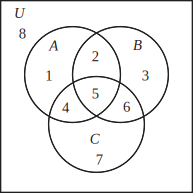
\includegraphics{figps-venn3.eps}
%\end{center}
%\end{figure}


\item Based on the Venn diagrams in Part (1), it appears that 
$A \cup \left( {B \cap C} \right) = \left( {A \cup B} \right) \cap \left( {A \cup C} \right)$.
\end{enumerate}



\subsection*{Progress Check~\ref{prog:usingalgebrasets}}
\begin{enumerate}
  \item Using our standard configuration for a Venn diagram with three sets, regions 1, 2, and 3 are the regions that are shaded for both 
$\left( {A \cup B} \right) - C$  and   $\left( {A - C} \right) \cup \left( {B - C} \right)$.
  \item \begin{align*}
\left( {A \cup B} \right) - C &= \left( {A \cup B} \right) \cap C^c &\text{(Theorem \ref{T:propsofcomplements})} \\
                              &= C^c  \cap \left( {A \cup B} \right) &\text{(Commutative Property)} \\
                              &= \left( C^c \cap A \right) \cup \left( C^c \cap B \right) &\text{Distributive Property} \\
                              &= \left( A \cap C^c \right) \cup \left( B \cap C^c \right) &\text{(Commutative Property)}\\
                              &= \left( A - C \right) \cup \left( B - C \right) &\text{(Theorem \ref{T:propsofcomplements})}
\end{align*}

\end{enumerate}

\hbreak

\endinput
